\documentclass{standalone}
\usepackage{tikz}
\usepackage{amsmath,amssymb,amsthm,mathtools}

\usetikzlibrary{3d,arrows.meta}
\usetikzlibrary{matrix, positioning}

\begin{document}

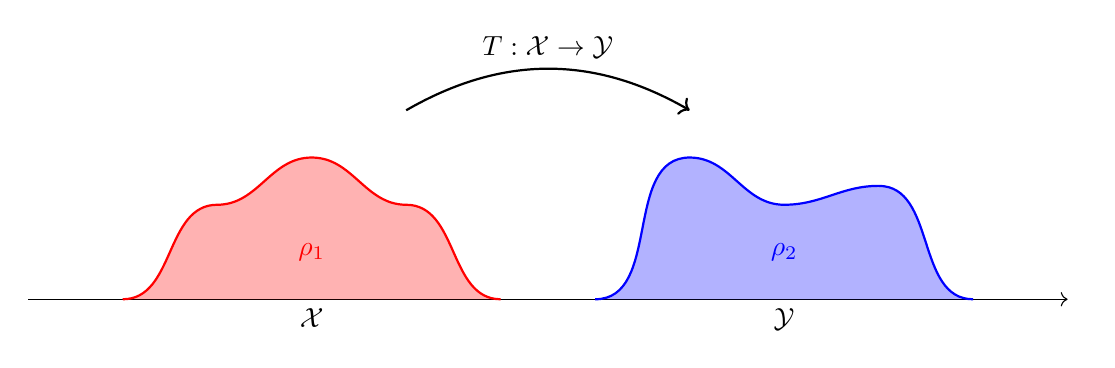
\begin{tikzpicture}[scale=1.2]
    \draw[->] (-1,0) -- (10,0) node[right] {};

    \draw[thick, red] (0,0) to[out=0, in=180] (1,1) to[out=0, in=180] (2,1.5) to[out=0, in=180] (3,1) to[out=0, in=180] (4,0);
    \fill[red, opacity=0.3] (0,0) to[out=0, in=180] (1,1) to[out=0, in=180] (2,1.5) to[out=0, in=180] (3,1) to[out=0, in=180] (4,0) -- (0,0);
    \node[red] at (2,0.5) {$\rho_1$};
    \node[below] at (2,0) {$\mathcal{X}$};

    \draw[thick, blue] (5,0) to[out=0, in=180] (6,1.5) to[out=0, in=180] (7,1) to[out=0, in=180] (8,1.2) to[out=0, in=180] (9,0);
    \fill[blue, opacity=0.3] (5,0) to[out=0, in=180] (6,1.5) to[out=0, in=180] (7,1) to[out=0, in=180] (8,1.2) to[out=0, in=180] (9,0) -- (6,0);
    \node[blue] at (7,0.5) {$\rho_2$};
    \node[below] at (7,0) {$\mathcal{Y}$};

    \draw[->, thick, bend left] (3,2) to node[midway, above] {$T:\mathcal{X}\to \mathcal{Y}$} (6,2);
\end{tikzpicture}

\end{document}